% !TeX spellcheck = en_US	


\documentclass[10pt,journal,compsoc]{IEEEtran}
\usepackage{graphicx}
\usepackage[ruled, linesnumbered]{algorithm2e}
\usepackage{url}
\usepackage{epstopdf}
\usepackage{indentfirst}
\usepackage[tight,footnotesize]{subfigure}
\usepackage{amsmath}
\usepackage{amssymb}
\usepackage{multirow}
\usepackage{color}
\usepackage{enumerate}

\newtheorem{Formula}{Formula}
\newtheorem{Lemma}{Lemma}
\newtheorem{Corollary}{Corollary}
\newtheorem{Property}{Property}
\newtheorem{Rule}{Rule}

% *** CITATION PACKAGES ***
\ifCLASSOPTIONcompsoc
\usepackage[nocompress]{cite}
\else
\usepackage{cite}
\fi


\begin{document}


\title{Checking Big Suffix and LCP Arrays by Probabilistic Methods}

\author{
	Yi~Wu,
	Ge~Nong,
	Wai~Hong~Chan,
	Ling~Bo~Han% <-this % stops a space
	\IEEEcompsocitemizethanks{
		\IEEEcompsocthanksitem Y. Wu, G. Nong (corresponding author) and L.~B.~Han are with the Department of Computer Science, Sun Yat-sen University, Guangzhou 510275, China. E-mails: wu.yi.christian@gmail.com, issng@mail.sysu.edu.cn, hanlb@mail2.sysu.edu.cn.
		
		\IEEEcompsocthanksitem Wai Hong Chan (corresponding author) is with the Department of Mathematics and Information Technology, The Education University of Hong Kong, Hong Kong. E-mail: waihchan@ied.edu.hk.
}}% <-this % stops a space
	
\IEEEtitleabstractindextext{%
\begin{abstract}

For full-text indexing of massive data, the suffix and LCP (longest common prefix) arrays have been recognized as the fundamental data structures, and there are at least two needs in practice for checking their correctness, i.e. program debugging and verifying the arrays constructed by probabilistic algorithms. In this paper, we propose two methods to check the suffix and LCP arrays in external memory by using a Karp-Rabin fingerprinting technique, where the checking result is wrong only with a negligible error probability. The first method checks the lexicographical order and the LCP-value of two neighboring suffixes in the given suffix array by computing and comparing the fingerprints of their LCPs. This idea is also employed in the second method to verify a subset of the given suffix and LCP arrays, from which then a copy of the final suffix and LCP arrays is produced following the induced sorting principle and compared with the given arrays for verification.


\end{abstract}

% Note that keywords are not normally used for peerreview papers.
\begin{IEEEkeywords}
	Suffix and LCP arrays verification, Karp-Rabin fingerprinting technique, external memory.
\end{IEEEkeywords}}


% make the title area
\maketitle

\IEEEdisplaynontitleabstractindextext

\IEEEpeerreviewmaketitle

\section{Introduction}\label{sec:introduction}

\subsection{Background} \label{sec:introduction:background}


Suffix and longest common prefix (LCP) arrays play an important role in various string processing tasks, such as data compression, pattern matching and genome assembly. In many applications, these two data structures make up the core part of a powerful full-text index, called enhanced suffix array~\cite{Abouelhodaa2004}, which is more space efficient than a suffix tree and applicable to emulating any searching functionalities provided by the latter in the same time complexity. The first algorithm for building suffix array in internal memory was presented in~\cite{Manber1993}. From then on, much more effort has been put on designing efficient constructors for suffix array~(SA) on different memory models~\cite{Karkkainen2003, Ko2003, Kim2003, Nong11, Dementiev2008, Ferragina2012, Manzini2004, Bingmann12, Karkkainen2014, Nong14, Nong15}. In respect of the research on LCP-array construction algorithms, the existing works can be classified into two categories with regard to the input requirements, where the algorithms from the first category compute both suffix and LCP arrays at the same time with the original text only~\cite{Fischer11, Bingmann12, Flick2015} and those from the second category carry out the computation by taking SA and/or Burrows-Wheeler transform (BWT) as additional input~\cite{Kasai2001,Karkkainen2009, Fischer11, Puglisi2008, Puglisi2008, Deo2013}. Among all, the algorithms designed by the induced sorting~(IS) principle take linear time and space to run and outperform previous arts on both internal and external memory models~\cite{Nong11, Karkkainen2014}. Recently, there appear some novel works that are competitive with the IS-based ones and even achieve better performance when adequate computation resources are available. These algorithms can maximize their throughput by making use of the multi-core CPUs and/or GPUs in computers~\cite{Osipov2012, Deo2013, Wang2015, Karkkainen2015, Karkkainen2016}. 

While the research on efficient construction of suffix and LCP arrays is evolving, the algorithms proposed recently are becoming more complicated than before. This reveals a need for program debugging because a program gives no guarantee that it has correctly implemented the underlying algorithm. As a common practice, a suffix or LCP checker is provided to check the correctness of a constructed array. For example, such a checker can be found in some software packages for SA-IS~\cite{Nong11}, eSAIS~\cite{Bingmann12}, DC3~\cite{Dementiev08} and so forth. In addition to help avoid implementation bugs, a checker is also demanded for an array constructed by a probabilistic algorithm~\cite{Bille2013}. In this case, the array is correctly constructed with a probability and hence must be verified by a checker to ensure its correctness. As far as we know, the work in~\cite{Burkhardt2003} describes the only SA checking method that can be found in the existing literature, and no efficient checking method for LCP array has been reported yet. In particular, there is currently no reported solution that can check both the suffix and the LCP arrays in external memory. This motivates our work here to design high-performance SA and LCP checkers for massive data.  
	
\subsection{Contribution}\label{sec:introduction:contribution}

Our contribution mainly includes two methods to probablistically verify the given suffix and LCP arrays. Method A checks the lexical order and LCP-value of two neighboring suffixes in SA by literally comparing the characters of their LCPs in pairs. For reducing the time complexity of a comparison between two sequences of characters, we use a Karp-Rabin fingerprinting technique to convert each sequence into a single integer, called fingerprint, and compare the fingerprints instead to check equality of these sequences. The algorithm for this method involves multiple scans and sorts on sets of $\mathcal{O}(n)$ fixed-size items. When implemented in external memory, it suffers from a space bottleneck owing to the large disk volume taken by each sort. 
To overcome the drawback, Method B first employs the fingerprinting technique to check a subset selected from the given suffix and LCP arrays, then it reuses the inducing process of an IS-based algorithm to produce the final suffix and LCP arrays from the verified subset and literally compares them with the input arrays to ensure the correctness of the latter. Our experiments indicate that the peak disk use of the program for the algorithm designed by Method B is only half as that of the program for the algorithm designed by Method A.

The remainder of this paper is organized as follows. We first describe the checking methods and their algorithmic designs in Sections~\ref{sec:method1} and~\ref{sec:method2}, and then evaluate the performance of our programs for the algorithms of these methods in Section~\ref{sec:experiment}. Finally, we present the concluding remarks in Section~\ref{sec:conclusion}. 



\section{Method A} \label{sec:method1}


\subsection{Preliminaries} \label{sec:method1:notations}

Given a string $x[0, n)$ drawn from an alphabet $\Sigma$, the suffix array of $x$, denoted by $sa$, is a permutation of $\{0, 1, ..., n - 1\}$ such that ${\sf suf}(sa[i]) < {\sf suf}(sa[j])$ for $i, j \in [0, n)$ and $i < j$, where ${\sf suf}(sa[i])$ and ${\sf suf}(sa[j])$ are two suffixes starting with $x[sa[i]]$ and $x[sa[j]]$, respectively. Particularly, we say ${\sf suf}(sa[j])$ is a lexical neighbor of ${\sf suf}(sa[i])$ if $|i - j| = 1$. The LCP array of $x$, denoted by $lcp$, consists of $n$ integers, where $lcp[0]=0$ and $lcp[i]$ records the LCP-value of ${\sf suf}(sa[i])$ and ${\sf suf}(sa[i - 1])$ for $i \in [1, n)$.


\subsection{Idea} \label{sec:method1:idea}

According to the definitions of $sa$ and $lcp$, we show in Lemma~\ref{lemma:1} the sufficient and necessary conditions for checking the given suffix and LCP arrays. Notice that the lexical order and the LCP-value of two suffixes in $x$ can be computed by literally comparing their characters from left to right. Because all the suffixes differ in length and end with a common character, there must exist $k \in [0, n)$ such that $x[i, i + k) = x[j, j + k)$ and $x[i + k] \ne x[j + k]$ for any $i, j \in [0, n)$ and $i \ne j$. This approach can be also applied to verifying the last two conditions in Lemma~\ref{lemma:1}, but it takes at worst $\mathcal{O}(n)$ character-wise comparisons for each pair of neighboring suffixes in $sa$ to compare the two substrings, that is the LCPs, indicated by their LCP-value.

\begin{Lemma} \label{lemma:1}
	Both $sa[0, n)$ and $lcp[0, n)$ are correct if and only if the following conditions are satisfied, for all $i \in [1, n)$:
	\begin{enumerate}[(1)]
		\item
		$sa$ is a permutation of $\{0, 1, \dots, n - 1\}$.
		\item
		$x[sa[i], sa[i] + lcp[i] - 1] = x[sa[i - 1], sa[i - 1] + lcp[i] - 1]$.
		\item
		$x[sa[i] + lcp[i]] > x[sa[i - 1] + lcp[i]]$. 	
	\end{enumerate}
\end{Lemma}

\begin{IEEEproof}
	Both the sufficiency and necessity are immediately seen from the definition of suffix and LCP arrays. Specifically, condition (1) demonstrates that all the suffixes in $x$ are sorted in $sa$, while conditions (2)-(3) indicate that the lexical order and the LCP-value of any two neighboring suffixes in $sa$ are both correct.
\end{IEEEproof}

An alternative is to exploit a perfect hash function~(PHF) to convert each substring into a single integer such that any two substrings have a common hash value if and only if they are literally equal to each other. This implies that we can compare the hash values instead to check equality of their corresponding substrings. The key point here is how to quickly calculate the hash values of $x[sa[i], sa[i] + lcp[i] - 1]$ and $x[sa[i - 1], sa[i - 1] + lcp[i] - 1]$ for all $i \in [1, n)$. Taking into consideration the high difficulty of finding a PHF to meet this requirement, we prefer using a Karp-Rabin fingerprinting function~\cite{Karp1987} to transform a substring into its integer form, called fingerprint. Specifically, suppose $L$ is a prime and $\delta$ is randomly chosen from $[1, L)$, the fingerprint ${\sf fp}(i, j)$ of a substring $x[i, j]$ can be calculated according to the formulas below as following: scan $x$ rightward to iteratively compute ${\sf fp}(0, k)$ for all $k \in [0, n)$ using Formulas~\ref{formula:1}-\ref{formula:2}, record ${\sf fp}(0, i - 1)$ and ${\sf fp}(0, j)$ during the calculation and subtract the former from the latter to obtain ${\sf fp}(i, j)$ using Formula~\ref{formula:3}.

\begin{Formula} \label{formula:1}
	${\sf fp}(0, -1) = 0$.
	
\end{Formula}

\begin{Formula} \label{formula:2}	
	${\sf fp}(0, i) = {\sf fp}(0, i - 1) \cdot {\delta} + x[i]\mod L$ for $i \ge 0$.
	
\end{Formula}

\begin{Formula} \label{formula:3}
	${\sf fp}(i, j) = {\sf fp}(0, j) - {\sf fp}(0 ,i - 1) \cdot {\delta}^{j - i + 1}\mod L$.
	
\end{Formula}

We point out that two equal substrings always share a common fingerprint, but the inverse is not true. Fortunately, it has been proved in~\cite{Karp1987} that the probability of a false match can be reduced to a negligible level by setting $L$ to a large value\footnote{This property is utilized in~\cite{Bille2013} to design a probabilistic algorithm for computing a sparse suffix array. }. This leads us to the conclusion in Corollary~\ref{corollary:1}.

\begin{Corollary} \label{corollary:1}
	Both $sa[0, n)$ and $lcp[0, n)$ are correct with a high probability given the following conditions, for all $i \in [1, n)$:
	
	\begin{enumerate}[(1)]
		\item
		$sa$ is a permutation of $\{0, 1, \dots, n - 1\}$.
		
		\item
		${\sf fp}(sa[i], sa[i] + lcp[i] - 1) = {\sf fp}(sa[i - 1], sa[i - 1] + lcp[i] - 1)$.
		
		\item
		$x[sa[i] + lcp[i]] > x[sa[i - 1] + lcp[i]]$.
	\end{enumerate}
\end{Corollary}

We show in Fig.~\ref{fig:example} an example for better understanding. Assume $L = 197$ and $\delta = 101$, lines 4-8 compute ${\sf fp}(0, p)$ iteratively according to Formulas~\ref{formula:1}-\ref{formula:2}. These values are used to compute the fingerprints for the target substrings. Consider the leftmost pair of neighboring suffixes in $sa$, that is ${\sf suf}(sa[0])$ and ${\sf suf}(sa[1])$, the substrings indicated by their LCP-value are $x[sa[0], sa[0] + lcp[1] - 1]$ and $x[sa[1], sa[1] + lcp[1] - 1]$, respectively. According to Formula~\ref{formula:3}, ${\sf fp}(sa[0], sa[0] + lcp[1] - 1)$ is equal to the difference between ${\sf fp}(0, sa[0])$ and ${\sf fp}(0, sa[0] + lcp[1] + 1)$, which have been calculated beforehand. In lines 10-12, we obtain the fingerprints for these two substrings and find that they are equal to each other. 

\begin{figure*}
	\centering
	\label{fig:example}
	\includegraphics[width = 0.8\textwidth]{example}
	\caption{An Example for Computing the Fingerprints for the LCPs of the Neighboring Suffixes in SA.}	
\end{figure*}

\subsection{Algorithm} \label{sec:method1:algorithm}

We first describe an algorithm for checking conditions in Corollary~\ref{corollary:1} on random access models, of which the core part is to check the lexical order and LCP-value for each pair of neighboring suffixes in $sa$ on-the-fly during the scan of $sa$ and $lcp$. This is done by using Formulas~\ref{formula:1}-\ref{formula:3} following our discussion in the previous subsection. As can be seen, two zero-initialized array, namely $fp$ and $mk$, are introduced to facilitate the checking process, where $fp$ is for storing the fingerprints of prefixes and $mk$ is for determining whether or not each number of $\{0, 1, ..., n - 1\}$ is present in $sa$.

\begin{enumerate}
	\item [S1]
	Scan $x$ rightward with $i$ increasing from $0$ to $n - 1$. For each scanned $x[i]$, compute ${\sf fp}(0, i)$ and assign the value to $fp[i]$.
	
	\item [S2]
	Scan $sa$ and $lcp$ rightward with $i$ increasing from $1$ to $n - 1$. For each scanned $sa[i]$ and $lcp[i]$, let $u = sa[i], v = lcp[i], w = sa[i - 1]$ and perform substeps (a)-(c) in sequence:
	
	\begin{enumerate}[(a)]
		\item
		Retrieve $fp[u - 1]$ and $fp[u + v - 1]$ from $fp$ to compute ${\sf fp}(u, u + v - 1)$. Set $mk[u]$ to $1$.
		
		\item
		Retrieve $fp[w - 1]$ and $fp[w + v - 1]$ from $fp$ to compute ${\sf fp}(w, w + v - 1)$.
		
		\item
		Check if ${\sf fp}(u, u + v - 1) = {\sf fp}(w, w + v - 1)$ and $x[u + v] > x[w + v]$.
		
		\item
		Set $mk[sa[0]] = 1$.
	\end{enumerate}

	\item [S3] Check if $mk[i] = 1$ for all $i \in [0, n)$.
	
\end{enumerate}

It is clear that the above algorithm consumes $\mathcal{O}(n)$ time and space when implemented in internal memory. However, if the two auxiliary arrays cannot be wholly accommodated into RAM during the execution of S2, it suffers from a performance degradation caused by frequent random accesses to disks. Assume that $x$, $sa$ and $lcp$ are stored in external memory, we design Algorithm~\ref{alg:1} for conducting these I/O operations in a disk-friendly way. The main idea is to first sort data in the order that they are visited and then access them by sequential reads and writes. To the end, our algorithm first scans $sa$ and $lcp$ to produce $ST_1, ST_2, ST_3$ and sorts their tuples by 1st component in ascending order at the very beginning (lines~\ref{alg:1:a}-\ref{alg:1:b}). Afterward, it iteratively computes the fingerprints of all the prefixes according to Formulas~\ref{formula:1}-\ref{formula:2} and assigns them to the sorted tuples as following (lines~\ref{alg:1:c}-\ref{alg:1:d}): when figuring out ${\sf fp}(0, i - 1)$, extract each tuple $e$ with $e.1st = i$ from $ST_1/ST_2/ST_3$, update $e$  with ${\sf fp}(0, i - 1)$, and then forward $e$ to $ST_1'/ST_2'/ST_3'$. Because the 1st component of the tuples in $ST_1$ constitute a copy of $sa$, the algorithm can check condition (1) in lines~\ref{alg:1:h}-\ref{alg:1:i} when scanning them in the sorted order. Finally, it sorts the updated tuples back to their original order (line~\ref{alg:1:e}) and visits them  sequentially to check conditions (2)-(3) following the same way of S2.  



\SetKwProg{Fn}{Function}{}{}

\begin{algorithm*}

	\caption{The Algorithm Based on Corollary~\ref{corollary:1}.}
	
	\label{alg:1}
	
	%\SetAlgoNoLine
	\Fn{{\sf CheckByFP}($x$, $sa$, $lcp$, $n$)}{
	
		$ST_1$ := $[(sa[i], i, null) | i \in [0, n)]$ \label{alg:1:a}
		
		$ST_2$ := $[(sa[i] + lcp[i + 1], i, null, null) | i \in [0, n - 1)]$
			
		$ST_3$ := $[(sa[i] + lcp[i], i, null, null) | i \in [1, n)]$
		
		sort tuples in $ST_1$, $ST_2$ and $ST_3$ by 1st component \label{alg:1:b}
		
		$fp := 0$  \label{alg:1:c}
		
		\For{$i \in [0, n]$}{
			
			\If{$ST_1.{\sf notEmpty}()$ {\sf and} $ST_1.{\sf top}().1st = i$}{~\label{alg:1:h}
				$e := ST_1.{\sf top}()$, $ST_1.{\sf pop}()$, $e.3rd := fp$, $ST_1'.{\sf push}(e)$
			}
			\Else{
				\Return false \hspace{5cm} // condition (1) is violated
			}~\label{alg:1:i}
			\While{$ST_2.{\sf notEmpty}()$ {\sf and} $ST_2.{\sf top}().1st = i$}{
				
				$e := ST_2.{\sf top}()$, $ST_2.{\sf pop}()$, $e.3rd := fp$, $e.4th := x[i]$, $ST_2'.{\sf push}(e)$
			}	
		
			\While{$ST_3.{\sf notEmpty}()$ {\sf and} $ST_3.{\sf top}().1st = i$}{
				
				$e := ST_3.{\sf top}()$, $ST_3.{\sf pop}()$, $e.3rd := fp$, $e.4th := x[i]$, $ST_3'.{\sf push}(e)$
			}	
		
			$fp := fp \cdot \delta + x[i] \! \mod \! P$
		} \label{alg:1:d}
		
		sort tuples in $ST_1$, $ST_2$ and $ST_3$ by 2nd component.  \label{alg:1:e}
		
		\For {$i \in [1, n - 1)$}{  \label{alg:1:f}
			
			$fp_1 := ST_1'.{\sf top}().3rd$, $ST_1'.{\sf pop}()$, $fp_2 := ST_2'.{\sf top}().3rd$, $ch_1 := ST_2'.{\sf top}().4th$, $ST_2'.{\sf pop}()$
			
			$\hat{fp_1} = fp2 - fp1 \cdot \delta^{lcp[i]} \! \mod \! P$ \label{alg:1:j}
		
		 	$fp_1 := ST_1'.{\sf top}().3rd$, $fp_3 := ST_2'.{\sf top}().3rd$, $ch_2 := ST_3'.{\sf top}().4th$, $ST_3'.{\sf pop}()$
			
			$\hat{fp_2} = fp3 - fp1 \cdot \delta^{lcp[i]} \! \mod \! P$	\label{alg:1:k}
			
			\If{$\hat{fp_1} \ne \hat{fp_2}$ {\sf or} $ch_1 \le ch_2$}{
				
				\Return false \hspace{5cm} // condition (2) or (3) is violated
			}	
		} \label{alg:1:g}

		\Return true
	}
	\end{algorithm*}

The last point to be mentioned here is how to obtain the value of $\delta^{lcp[i]}$ quickly when computing $\hat{fp_1}$ and $\hat{fp_2}$ in lines~\ref{alg:1:j} and~\ref{alg:1:k}. One method is to keep a lookup table in internal memory to store $\delta^{lcp[i]}$ for all $i \in [0, n)$. This method can answer the question in constant time, but it is space-consuming and 
impractical to use when the table is bigger than the memory bank capacity. We provide another method that returns the answer in $\mathcal{O}(\lceil \log2^n \rceil)$ time using $\mathcal{O}(\lceil \log2^n \rceil)$ internal memory space. Specifically, suppose $e$ is an integer from $[0, n)$, it can be decomposed into the form of $\Sigma_{i = 0}^{\lceil \log2^n \rceil}{k_i \cdot 2^i}$, where $k_0, k_1, ..., k_{\lceil \log2^n \rceil}$ are determined by performing at most $\lceil \log2^n \rceil$ divisions. Hence, we have $\delta^e = \Pi_{i = 0}^{\lceil \log2^n \rceil}{\delta}^{k_i \cdot 2^i}$ by replacing $e$ with its decomposition, where the expression on the right side of the equation can be easily computed with $\{{\delta}^{1}, {\delta}^{2}, \dots, {\delta}^{2^{\lceil \log2^n \rceil}} \}$ already known.

\subsection{Analysis} \label{sec:method1:analysis}


Algorithm~\ref{alg:1} is I/O-intensive, it performs multiple scans and sorts on the arrays of $\mathcal{O}(n)$ fixed-size tuples residing on disks. Given an external memory model with RAM size $M$, disk size $D$ and block size $B$, all are in words, the time and I/O complexities for each scan are $\mathcal{O}(n)$ and $\mathcal{O}(n / B)$, respectively, while those for each sort are $\mathcal{O}(n\log_{M/ B}(n / B))$ and $\mathcal{O}((n / B)\log_{M / B}(n / B))$, respectively~\cite{Arge2013}. This algorithm reaches its peak disk use when sorting tuples in lines~\ref{alg:1:b} and~\ref{alg:1:e}. A trick for reducing	the space requirements is to compute the fingerprints of prefixes specified in $ST_1$, $ST_2$ and $ST_3$, respectively. However, our experimental study in Section~\ref{sec:experiment} shows that Algorithm~\ref{alg:1} is still rather space hungry, its peak disk use is 40 bytes per input character. In the next section, we will describe an alternative checking method based on the induced-sorting principle. Compared with Algorithm~\ref{alg:1}, the program for our algorithm designed by this method only takes half space on real-world datasets.

\section{Method B} \label{sec:method2}

\subsection{Preliminaries} \label{sec:method2:preliminaries}

We introduce some symbols and notations used in the following presentation.

{\em Character and suffix classification.} All the characters in $x$ are classified into three types, namely L-, S- and S*-type. In detail, $x[i]$ is L-type if (1) $i = n - 1$ or (2) $x[i] > x[i + 1]$ or (3) $x[i] = x[i + 1]$ and $x[i + 1]$ is L-type; otherwise, $x[i]$ is S-type. Further, if $x[i]$ and $x[i + 1]$ are respectively S- and L-type, then $x[i]$ is also an S*-type character. Moreover, a suffix is L-, S- or S*-type if its heading character is L-, S-, or S*-type, respectively.

{\em Suffix and LCP buckets.} Suppose $sa$ is correct, all the suffixes in $sa$ are naturally partitioned into multiple buckets and those of a common heading character are grouped into a single bucket that occupies a contiguous interval in $sa$. Each bucket can be further divided into two sub-buckets, where the left and right parts only contain L- and S-type suffixes, respectively. For short, we use ${\sf sa\_bkt}(c)$ to denote the bucket storing suffixes starting with character $c$ and ${\sf sa\_bkt_L}(c)/{\sf sa\_bkt_S}(c)$ to denote its left/right sub-bucket. Accordingly, $lcp$ can be also split into multiple buckets, where ${\sf lcp\_bkt}(c)/{\sf lcp\_bkt_L}(c)/{\sf lcp\_bkt_S}(c)$ stores the LCP-values of suffixes in ${\sf sa\_bkt}(c)/{\sf sa\_bkt_L}(c)/{\sf sa\_bkt_S}(c)$.

{\em Suffix and LCP arrays for S*-type suffixes.} Given that the number of S*-type suffixes is $n_1$, $sa^*[0, n_1)$ stores all the S*-type suffixes and arrange them in lexical order, while the $(i + 1)$-th item of $lcp^*[0, n_1)$ records the LCP-value of ${\sf suf}(sa^*[i])$ and ${\sf suf}(sa^*[i - 1])$.

\subsection{Idea} \label{sec:method2:idea}

The induced sorting principle has been employed to invent efficient algorithms for constructing suffix and LCP arrays on both internal and external memory models. These algorithms mainly consist of a reduction phase for computing $sa^*$ and $lcp^*$, followed by an induction phase for inducing $sa$ and $lcp$ from $sa^*$ and $lcp^*$. Given that $sa^*$ and $lcp^*$ are already known, we can directly construct the suffix and LCP arrays by calling the inducing process of any existing IS-based construction algorithm. This enlightens us to design a checker following Lemma~\ref{lemma:2}. 
	
\begin{Lemma} \label{lemma:2}
Both $sa[0, n)$ and $lcp[0, n)$ are correct if and only if the conditions below are satisfied:

\begin{enumerate}[(1)]
	\item
	$sa^*$ and $lcp^*$ are both correct.
	\item
	$sa = sa'$ and $lcp = lcp'$, where $sa'$ and $lcp'$ are induced from $sa^*$ and $lcp^*$ by calling the inducing process of any existing IS-based construction algorithm.
\end{enumerate}
\end{Lemma}

Similar to Method A, we can employ the fingerprinting technique to probablistically check the correctness of $sa^*$ and $lcp^*$. Based on this idea, we describe in the subsequent paragraphs an external-memory algorithm for checking the conditions in Corollary~\ref{corollary:2}.

\begin{Corollary} \label{corollary:2}
Both $sa[0, n)$ and $lcp[0, n)$ are correct with a high probability given the following conditions, for $i \in [0, n)$, $\{j, k\} \in [1, n_1)$ and $j \ne k$:
	
\begin{enumerate}[(1)]
	\item
	$sa^*[j] \ne sa^*[k]$.
	\item
	${\sf fp}(sa^*[j], sa^*[j] + lcp^*[j] - 1) = {\sf fp}(sa^*[j - 1], sa^*[j - 1] + lcp^*[j] - 1)$.
	\item
	$x[sa^*[j] + lcp^*[j]] > x[sa^*[j - 1] + lcp^*[j]]$.
	\item
	$sa[i] = sa'[i]$ and $lcp[i] = lcp'[i]$, where $sa'$ and $lcp'$ are induced from $sa^*$ and $lcp^*$ by calling the inducing process of an existing IS-based construction algorithm.
\end{enumerate}

\end{Corollary}


\subsection{Algorithm} \label{sec:method2:algorithm}

The first step of Algorithm~\ref{alg:2} is to compute and verify $sa^*$ and $lcp^*$. According to the definition, $sa^*$ can be produced by sequentially retrieving the S*-type suffixes from $sa$ while the LCP-value of two successive S*-type suffixes in $sa$, say ${\sf suf}(sa[i])$ and ${\sf suf}(sa[j])$, is equal to the minimal of $\{lcp[i + 1], ..., lcp[j - 1], lcp[j]\}$. Hence, the proposed algorithm first sorts all the suffixes in $sa$ by their starting positions~(lines~\ref{alg:2:a}-\ref{alg:2:b}) and then scans $x$ only once to pick out the S*-type suffixes~(lines~\ref{alg:2:c}-\ref{alg:2:d}). After that, it puts these S*-type suffixes back in their lexical order and outputs them one by one to generate $sa^*$~(lines~\ref{alg:2:g}-\ref{alg:2:h}). Meanwhile, it calculates the LCP-value for each pair of neighboring suffixes in $sa^*$ by tracing the minimal over an interval of $lcp$ specified by the two suffixes. Notice that, we check condition (1) in Corollary~\ref{corollary:2} during the time when visiting the suffixes in position order (lines~\ref{alg:2:e}-\ref{alg:2:f}) and conditions (2)-(3) by calling Algorithm~\ref{alg:1} with $sa^*$ and $lcp^*$ as input. Suppose $sa^*$ and $lcp^*$ are both correct, then Algorithm~\ref{alg:1} invokes the inducing process of an existing construction algorithm to induce $sa'$ and $lcp'$, which are a copy of the final suffix and LCP arrays, from the two verified arrays~(line~\ref{alg:2:k}) and literally compares them with $sa$ and $lcp$ to complete the whole checking process~(lines~\ref{alg:2:l}-\ref{alg:2:m}).

\begin{algorithm*}
	
	\caption{The Algorithm Based on Corollary~\ref{corollary:2}.}
	
	\label{alg:2}
	
	%\SetAlgoNoLine
	\Fn{{\sf CheckByIS}($x$, $sa$, $lcp$, $n$)}{	
	
	$ST_1$ := $[(sa[i], i, null) | i \in [0, n)]$ \label{alg:2:a}
		
	sort tuples in $ST_1$ by 1st component \label{alg:2:b}
	
	$pos := -1$ \label{alg:2:c}
	
	\For{$i \in (n, 0]$}{
	
		$e := ST_1.{\sf top}()$, $ST_1.{\sf pop}()$
		
		\If{$x[i]$ is S*-type}{ \label{alg:2:e}
			
			\If{$pos \ge e.1st$}{
			
				\Return false  \hspace{1cm} // condition (1) is violated
			}
		
			$ST_2.{\sf push}(e)$, $pos := e.1st$
		}\label{alg:2:f}
	} \label{alg:2:d}

	sort tuples in $ST_2$ by 2nd component \label{alg:2:g}
	
	$i := 0$, $j := 0$, $lcp_{min} := max\_val$
	
	\While{$ST_2.{\sf NotEmpty()}$}{
	
		$e := ST_2.{\sf top}()$, $ST_2.{\sf pop}()$
	
		\While {true} {
			
			$lcp_{min} := {\sf min}(lcp_{min}, lcp[i])$
			
			\If {$e.2nd = i$} {
			
				$sa^*[j] := e.1st$, $lcp^*[j] := lcp_{min}$, $j := j + 1$, $i:= i + 1$
				
				\textbf{break}
			}
			
			$i:= i + 1$
		}
	
		$lcp_{min} := max\_val$
	} \label{alg:2:h}
	
	\If{${\sf CheckByFP}(x, sa^*, lcp^*, lcp^*.{\sf size}()) = false$}{  \label{alg:2:i}
	
		\Return false;  \hspace{1cm} // conditions (2) or (3) is violated
	}\label{alg:2:j}

	$(sa', lcp') := {\sf InducingProcess}(x, sa^*, lcp^*)$ \label{alg:2:k}
	
	\For{$i \in [0, n)$}{\label{alg:2:l}
	
		\If{$sa[i] \ne sa'[i] \parallel lcp[i] \ne lcp'[i]$}{
		
			\Return false	// condition (4) is violated
		}	
	}\label{alg:2:m}

	\Return true
}
\end{algorithm*}

Assume that the alphabet $\Sigma$ is of a constant size, we can check $sa$ and $lcp$ without producing a copy of the final suffix and LCP arrays in Algorithm~\ref{alg:2}. The idea is to compare the induced suffix/LCP items with their corresponding items in $sa/lcp$ during the inducing process. Specifically, when a suffix/LCP item $v_1$ is induced into a bucket, we check if it is equal to the corresponding item $v_2$ in $sa/lcp$. If $v_1 = v_2$, then $v_2$ is correct and we can further use it to induce the lexical order and LCP-value of its preceding suffix later. The key point here is how to retrieve items from $sa/lcp$ quickly. This can be done by performing sequential I/O operations when we provide a read pointer together with a buffer for each suffix/LCP sub-bucket. We show more details of the adapted inducing process as below, where $c \in [0, \Sigma)$ and $lp_1/lp_2$ and $sp_1/sp_2$ are read pointer arrays for retrieving items from the L-type/S-type sub-buckets in $sa$ and $lcp$.

\begin{enumerate}
	\item [S1]
	\begin{enumerate}[(a)]
		\item 
		Let $lp_1[c]$ and $lp_2[c]$ point to the leftmost items of ${\sf sa\_bkt_L}(c)$ and ${\sf lcp\_bkt_L}(c)$, respectively.
		\item 
		Scan $sa/lcp$ rightward to induce L-type suffixes and their LCP-values. For each induced suffix $p$ (with a heading character $c_0$) and its LCP-value $q$: (1) check if $p = lp_1[c_0]$ and $q = lp_2[c_0]$; (2) let $lp_1[c_0]$ and $lp_2[c_0]$ point to the next items on the right side.
	\end{enumerate}
	\item [S2]
	\begin{enumerate}[(a)]
		\item 	
		Let $sp_1[c]$ and $sp_2[c]$ point to the rightmost items of ${\sf sa\_bkt_S}(c)$ and ${\sf lcp\_bkt_S}(c)$, respectively.
		\item 	
		Scan $sa/lcp$ leftward to induce S-type suffixes and their LCP-values. For each induced suffix $p$ (with a heading character $c_0$) and its LCP-value $q$: (1) check if $p = sp_1[c_0]$ and $q = sp_2[c_0]$; (2) let $sp_1[c_0]$ and $sp_2[c_0]$ point to the next items on the left side.
	\end{enumerate}
\end{enumerate}


\subsection{Analysis} \label{sec:method2:analysis}

Algorithm~\ref{alg:2} mainly consists of two parts, where the first part for checking $sa^*$ and $lcp^*$ can be implemented within sorting complexity and the second part for checking $sa$ and $lcp$ can be implemented in linear time under the condition that $|\Sigma| = \mathcal{O}(1)$. As demonstrated in Section~\ref{alg:2}, the peak disk use of our program for Algorithm~\ref{alg:2} is around 20n and it has a similar performance compared to that for Algorithm~\ref{alg:1} in terms of time and I/O volume.

\section{Experiments} \label{sec:experiment}

\subsection{Setup} \label{sec:experiment:setup}

The experimental platform is a work station equipped with an Intel Xeon E3-1220 V2 CPU, 4GiB RAM and 500GiB HD. To achieve high I/O efficiency, the algorithms proposed in the previous sections are implemented using the external-memory containers provided by the STXXL library~\cite{Dementiev2007}. Our programs are compiled by gcc/g++ 4.8.4 with -O3 options under ubuntu 14.04 64-bit operating system. For analysis, we evaluate the performance on real-world datasets listed in Table~\ref{tbl:1} by investigating the following three measurements normalized by the size of input string:

\begin{itemize}
	
	\item RT: running time, in nanoseconds. Measured using the Linux 'time' command.
	
	\item PDU: peak disk use of external memory, in bytes.
	
	\item IOV: amount of data read from and write to external memory, in bytes.
	
\end{itemize}
	
%Table
\renewcommand\arraystretch{1.3}
\begin{table*}[!t]
	\caption{Corpus, $n$ in Gi, 1 byte per character}
	\label{tbl:1}
	\centering
	\begin{tabular}{|l|c|c|p{10cm}|}
		\hline
		Corpora & \multicolumn{1}{c|}{$n$} & \multicolumn{1}{c|}{$\|\Sigma\|$} & Description \\\hline
		enwiki & 8 & 256 & The 8-GiB prefix of an XML dump of English Wikipedia, available at \url{https://dumps.wikimedia.org/enwiki}, dated as 16/05/01. \\\hline	
		uniprot & 2.5 & 96 & UniProt Knowledgebase, available at \url{ftp://ftp.expasy.org/databases/.../complete}, dated as 16/05/11. \\\hline
		proteins & 1.1 & 27 & Swissprot database, available at \url{http://pizzachili.dcc.uchile.cl/texts/protein}, dated as 06/12/15. \\\hline
	\end{tabular}
\end{table*}

\subsection{Result} \label{sec:experiments:result}

Fig.~\ref{fig:cmp1} demonstrates the performance comparison between the programs for Algorithms~\ref{alg:1} and~\ref{alg:2}. As depicted,







The speed gap between them is mainly due to the difference in their I/O efficiencies. Specifically, the I/O volume of ProgB is 190$n$ in average, while that of ProgA is kept at 155$n$ for different corpora. Notice that, although Algorithm~\ref{alg:3} reuses Algorithm~\ref{alg:1} to check $sa_{\sf LMS}$ and $lcp_{\sf LMS}$, the consumption for the verification of $sa_{\sf LMS}$ and $lcp_{\sf LMS}$ in ProgB is at most half of ProgA because the number of LMS suffixes is no more than $\frac{1}{2}n$. It can be also observed that both programs are insensitive to the input corpus in terms of the space requirement. In details, the peak disk uses of ProgA and ProgB are respectively 26$n$ and 40$n$ on the three corpora.

We also investigate the performance trend of the two programs on the prefix of "enwiki" with the length varying on $\{1, 2, 4, 8\}$ GiB. Figure~\ref{fig:performance_analysis2} illustrates that, as the prefix length increases, a performance degradation occurs to ProgB in both time and I/O efficiencies, but the fluctuation of ProgA can be ignored.

%figure
\begin{figure}[htbp!]
	\centering
	\subfigure{
		\label{subfig:pdu_cmp}
		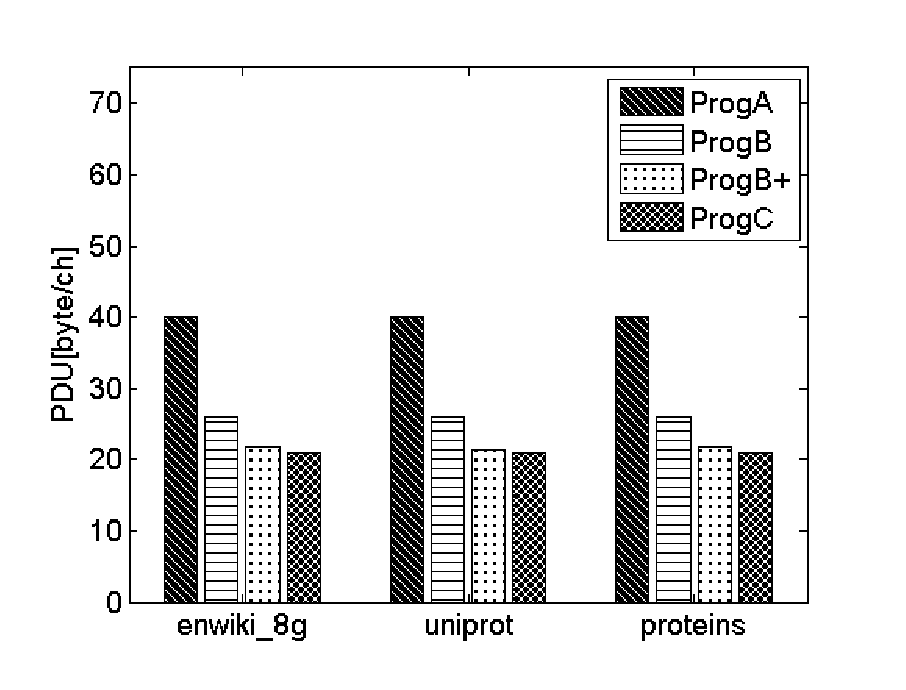
\includegraphics[width = 0.8\columnwidth]{pdu_cmp}
	}
	\hfil
	\subfigure{
		\label{subfig:iov_cmp}
		\includegraphics[width = 0.8\columnwidth]{io_cmp}
	}
	\hfil
	\subfigure{
		\label{subfig:ct_cmp}
		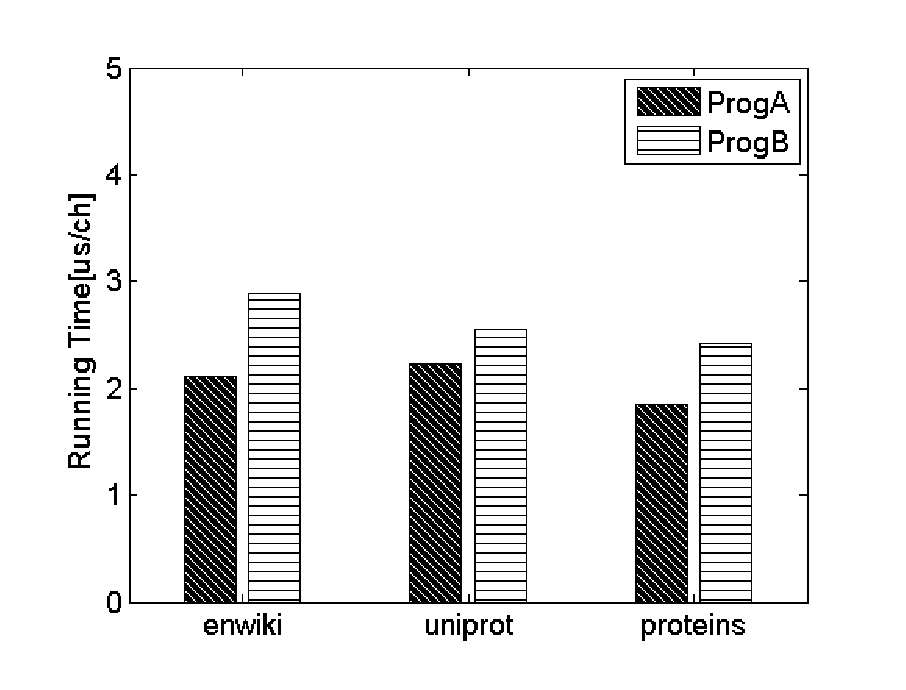
\includegraphics[width = 0.8\columnwidth]{ct_cmp}
	}
	\caption{Experimental results for various corpora.}
	\label{fig:performance_analysis}
\end{figure}

%figure
\begin{figure}[htbp!]
	\centering
	\subfigure{
		\label{subfig:pdu_cmp2}
		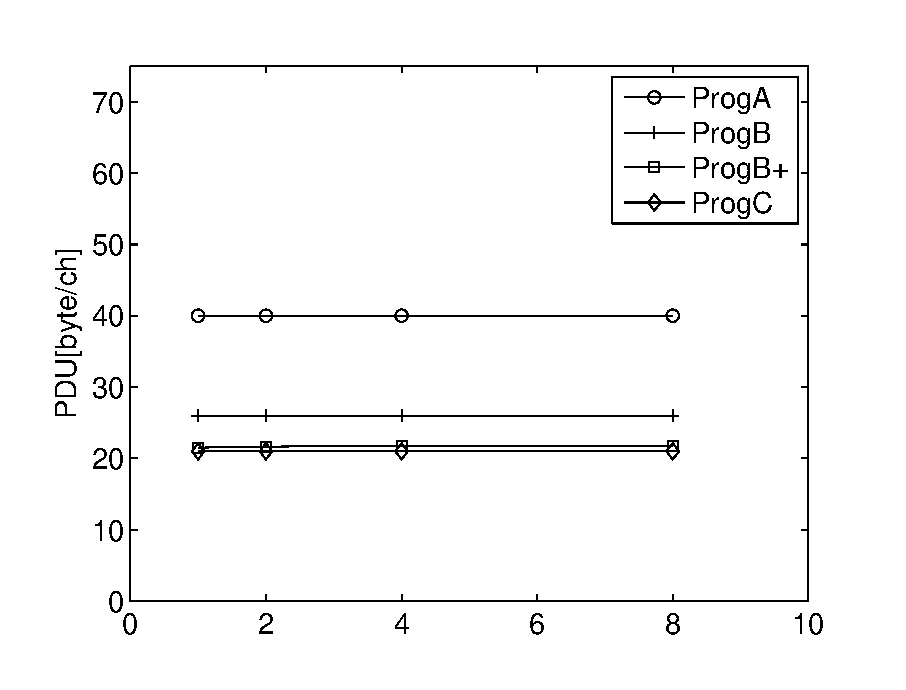
\includegraphics[width = 0.8\columnwidth]{pdu_cmp2}
	}
	\hfil
	\subfigure{
		\label{subfig:iov_cmp2}
		\includegraphics[width = 0.8\columnwidth]{io_cmp2}
	}
	\hfil
	\subfigure{
		\label{subfig:ct_cmp2}
		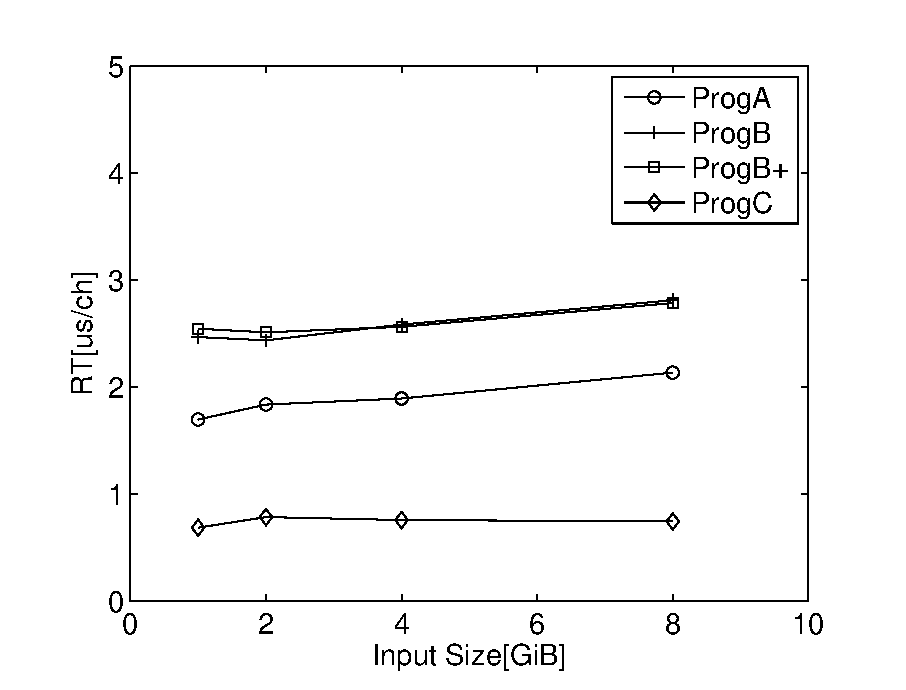
\includegraphics[width = 0.8\columnwidth]{ct_cmp2}
	}
	\caption{Experimental results for prefixes of "enwiki".}
	\label{fig:performance_analysis2}
\end{figure}
	
	\subsection{Discussion}
	
	It is identified that both programs heavily rely on the performance of the external memory sorter in use. A potential candidate for improving their speed is to adapt a GPU-based multi-way sorter~(e.g.,~\cite{Leischner2010, Davidson2012}) for sorting massive data using external memory. By the aid of these fast sorting algorithms, the throughputs of the programs are expected to nearly approach the I/O bandwidth. Besides, the first two steps of Algorithm~\ref{alg:1} are independent of each other and thus can be executed in parallel for acceleration. This technique can be also applied to check the suffix and LCP arrays of the LMS suffixes in Algorithm~\ref{alg:3}.
	
	Currently, for Algorithm~\ref{alg:3}, step 2 constitutes the space bottleneck. It is worthy of mentioning that this step produces a copy of the suffix and LCP array during the inducing and checking processes. Actually, given that $\Sigma$ is of a constant size and $sa/lcp$ are known already, we can simply scan the input $sa/lcp$ to perform the inducing process and compare each induced suffix/LCP value with that in the given $sa/lcp$ to perform the checking process, resulting in less space consumption. To the end, we must maintain a read pointer for each suffix/LCP bucket in $sa/lcp$ to scan elements in sequence.
	
\section{Conclusions} \label{sec:conclusion}

In this article, we propose two methods for probablistically checking the give suffix and LCP arrays using external memory. According to the experimental results, our program for Method A has a better performance than that for Method B with respect to the running time and I/O volume by about 20 percent, while the peak disk use of the latter is about 26/40=0.65 as that of the former and can be further reduced to around 21n without a sacrifice in the time and I/O effciency. We think these two methods could potentially be a xxxx .	 




% Bibliography
\bibliographystyle{IEEEtran}
\bibliography{IEEEabrv,bibfile}
	
\end{document}


We are intended for ....

put emphasis on

with the same ease as when

The biggest difference between two is that ...

Toward the end, ...

they are designed to be both easy to interpret on ... and easily traslated into ... (they are designed to be easily implemented in classic external memory models)

Having a ... eliminates .... (random accesses), access ordering

Not only are ..., but 

The fingerprints are calculated on the fly during the scan of x ...

become so good that they are competitive with ...., and in some cases, even outperform them ...

concurrent programming is needed to make sure ....

designed to adapt to an evolving environment

most importantly

exchanges data between the computer presenting the applet and the computer serving it.

carries out sophisticated calculations

Presumably because

make ... capable of ...

greatly improve ... , it was still rather limited, though.


additional performance improvements

close the chapter with ...

gain

which pose ...

integrate with

In this chapter, we will ... how to ... and how to ...


we prefer the comfort of an integrated development environment, ( prefer the low cost of fingerprinting techinques)

space-hungry


begin exploring ... by ...

commnuicate the monmentous advances

extremely simple

check each number is present in the suffix array.

go into much more greater details

stand-alone algorithms for computing suffix arrays only and has been reused to 

invoke/call


the mechanics of ...

If you have done sth, then when you do sth, you end up with ...

depend on the machine on which you will be running the java code ...


alleviate



The second method is invented to overcome the drawback of 

in place of

as to/about

as far as

assign to a variable

stated goals

intermediate steps

tied to the behavior of 

an assortment of 

following the footsteps of 

characters in the input string are processed from left to right

in greater detail




































